%% question-1.tex
%%

%% ==============================
\subsection{Diagramme de classe minimaliste du jeu}
\label{sec:question-1}
%% ==============================

Voici, un diagramme de classe UML qui fixe les éléments principaux du jeu, c'est à dire le jeu en lui même, les joueurs, avatars , les matchs , les rencontres et les mondes.

Le Jeu rassemble des joueurs, qui sauvegardent des avatars. Il possède des match qui sont constitués de rencontres qui on lieu dans des mondes. Mondes possédés par le Jeu.

\begin{figure}[h!]
	\centering
	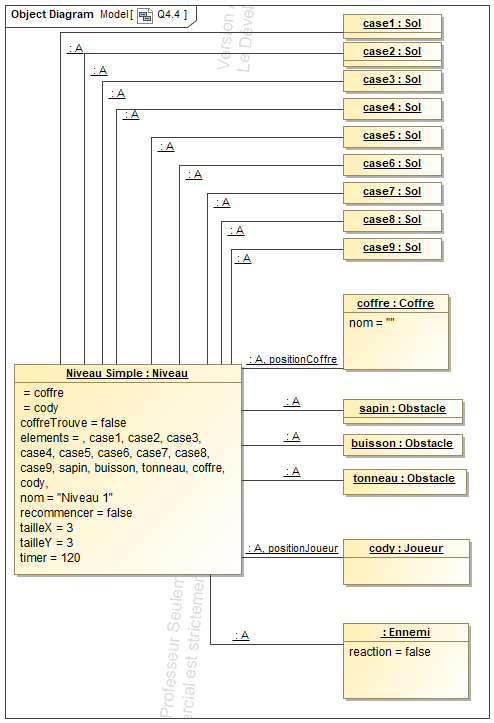
\includegraphics[width=250pt]{assets/Jeu_minimalist}
	\caption{Diagramme de classe des éléments principaux du jeu}
	\label{fig:diagrammeclassebase}
\end{figure}

\newpage